\begin{theorem}[Pairwise information has a sharp optimization penalty]\label{thm:pairwise-optimum}
Let $b\ge3$ be an integer, $H\ge0$, $S>0$, and $\lambda\ge0$.
For $n=b+1$ labeled leaves and internal arities $2,\ldots,b$, define
\begin{align*}
 J_D(T;\lambda)&=\lambda W(T)\\
 &\quad+\E_{U\sim D}\sum_{v\in\operatorname{int}(T)}c(d_v)
       \ind\{G(v)\cap U\ne\varnothing\}.
\end{align*}
There are distributions $P,Q$ with identical singleton and pairwise
probabilities but disjoint globally optimal tree sets, over every feasible
shape and leaf permutation. With $W_2=2H+S(b+2)$,
\begin{align}
 J_P^*&=(1+\lambda)W_2-(H+3S)/4,\label{eq:general-p}\\
 J_Q^*&=(1+\lambda)W_2-(H+2S)/4.\label{eq:general-q}
\end{align}
Any deterministic selector observing only those exact pairwise summaries has
worst-case regret at least $S/4$. The sharp randomized minimax regret is
\begin{equation}\label{eq:minimax-pairwise}
 \frac{S(H+2S)}{4(H+3S)}.
\end{equation}
Sibling orders are treated as equivalent.
\end{theorem}
\begin{proof}
Append $b-2$ anchor leaves, present in every event, to the two three-leaf
parity laws of Proposition~\ref{prop:pairwise}. Every singleton and pairwise
probability agrees, including anchor/parity pairs. An anchor-containing
node is always touched; a node containing only parity leaves is touched
with probability at least $3/4$.

If $I$ is the number of internal nodes, edge counting gives
$W(T)=I(H+S)+Sb$, and the arity cap implies $I\ge2$.
At most two internal nodes contain only the three parity leaves. If there
are two, both are binary; if there is one, its arity is at most three.
Their total price is at most $2c(2)$. Thus for either law and $I\ge3$,
\[
 J_D(T;\lambda)\ge(1+\lambda)W(T)-c(2)/2.
\]
A tree with two internal nodes and a parity-pair child costs
$(1+\lambda)W_2-c(2)/4$ under either law. Every $I\ge3$ lower bound exceeds
that pair tree by at least
\[
 (1+\lambda)(H+S)-c(2)/4
 = (3H+2S)/4+\lambda(H+S)>0.
\]
Such trees are componentwise dominated. With $I=2$, a child containing an
anchor is also dominated by a parity pair. The remaining choices are a
parity pair or the full parity triple. A pair is missed with probability
$1/4$ under either law. The triple is missed with probability $1/4$ under
$P$ and zero under $Q$. Since $c(3)>c(2)$, $P$ uniquely chooses the triple,
whereas $Q$ chooses any of its three pairs. This proves
Equations~\eqref{eq:general-p}--\eqref{eq:general-q}, including construction.

A pairwise-only rule receives identical inputs in both worlds. All other
tree classes are dominated, so a randomized rule need only choose the triple
with probability $q$ and a pair otherwise. Its two regrets are
\[
 r_P(q)=S(1-q)/4,\qquad r_Q(q)=(H+2S)q/4.
\]
The best deterministic choice is a pair, giving worst-case regret $S/4$.
Equating the two affine regrets gives $q^*=S/(H+3S)$ and
Equation~\eqref{eq:minimax-pairwise}. This mixture attains the lower bound.
\end{proof}

The result covers every affine positive-slot price and every fanout at least
three; it is not specific to the artifact's selected byte constants. It
concerns an interface exposing exact population pairwise summaries.
It does not assert equivalence of finite-sample statistical experiments:
joint fluctuations of empirical summary vectors can retain higher-order
information. It neither bounds a method
that retains full waves nor establishes the prevalence of such laws in
software executions. The events describe persistent refresh; a partial
event is not asserted to be a complete strict verification epoch.

\begin{figure}[t]\centering
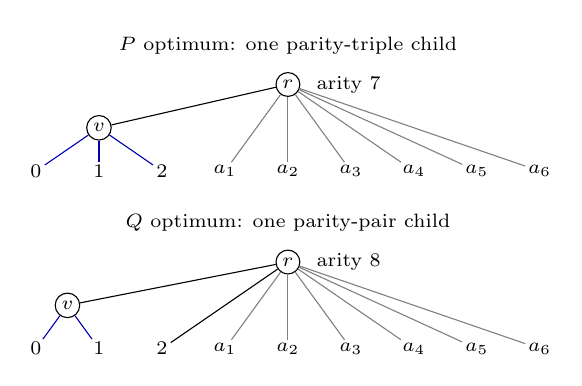
\begin{tikzpicture}[x=.8cm,y=.55cm,every node/.style={font=\scriptsize},
 root/.style={circle,draw,inner sep=1.3pt}, leaf/.style={inner sep=1pt}]
\node at (4,2.9) {$P$ optimum: one parity-triple child};
\node[root] (pr) at (4,2) {$r$};
\node[root] (pt) at (1,1) {$v$};
\node[right] at (4.3,2) {arity 7};
\foreach \x/\lab in {0/0,1/1,2/2,3/a_1,4/a_2,5/a_3,6/a_4,7/a_5,8/a_6}{
 \node[leaf] (p\x) at (\x,0) {$\lab$};}
\draw (pr)--(pt);
\foreach \x in {0,1,2}{\draw[blue!70!black] (pt)--(p\x);}
\foreach \x in {3,...,8}{\draw[gray] (pr)--(p\x);}
\node at (4,-1.2) {$Q$ optimum: one parity-pair child};
\node[root] (qr) at (4,-2.1) {$r$};
\node[root] (qt) at (.5,-3.1) {$v$};
\node[right] at (4.3,-2.1) {arity 8};
\foreach \x/\lab in {0/0,1/1,2/2,3/a_1,4/a_2,5/a_3,6/a_4,7/a_5,8/a_6}{
 \node[leaf] (q\x) at (\x,-4.1) {$\lab$};}
\draw (qr)--(qt);
\foreach \x in {0,1}{\draw[blue!70!black] (qt)--(q\x);}
\draw (qr)--(q2);
\foreach \x in {3,...,8}{\draw[gray] (qr)--(q\x);}
\end{tikzpicture}
\caption{Nine-leaf witness for Theorem~\ref{thm:pairwise-optimum}, with
$H=512,S=320,b=8$. The six anchors $a_i$ are distinct always-present
leaves, each a separate root child. Grouping the parity triple costs
3,856/4,224 refresh bytes under $P/Q$; grouping a pair costs 3,936
under either law. Construction adds 4,224 bytes to both trees.}
\label{fig:pairwise-witness}
\end{figure}


At these prices the deterministic penalty is 80 bytes; randomized minimax
regret is $1440/23\simeq62.609$ bytes, attained by choosing the triple with
probability $5/23$. Integer byte counts are the implementation case; the
theorem also allows real prices. Its zero-header boundary does not change
the serializer's stricter positive-header validation.

An independently implemented exact rational reference checks 39 parameter
cases, including zero headers, fractional construction and header-dominated
prices. It imports no HACT objective or optimizer. The nine-leaf case visits
511 nonempty subset subproblems and 115,462 candidate partitions \emph{across
those subproblems}; it finds one $P$ optimum and three $Q$ optima. Twenty-three
tests include independently listed four-leaf trees and deliberate formula
corruption. These are analytical checks, not additional software workloads.
